\documentclass[a4paper,12pt]{article}
\usepackage{times}
\usepackage[francais]{babel}
\usepackage[utf8]{inputenc}
\usepackage[T1]{fontenc}
\usepackage{amsmath}
\usepackage{amssymb}
\usepackage{graphicx}
\usepackage{pdfpages}
\usepackage{pdflscape}
\usepackage{listings}
\usepackage{longtable}
\usepackage{hyperref}
\lstset{literate=
{é}{{\'e}}1
{è}{{\`e}}1
{ê}{{\^e}}1
{à}{{\`a}}1
{â}{{\^a}}1
}
\lstset{language=C++,
                basicstyle=\footnotesize,
                keywordstyle=\footnotesize\color{blue},
                otherkeywords={override,nullptr}
}
\definecolor{orange}{rgb}{0.8,0.4,0.0}
\definecolor{darkblue}{rgb}{0.0,0.0,0.6}
\definecolor{cyan}{rgb}{0.0,0.6,0.6}
\lstdefinelanguage{JSON}
{
  basicstyle=\normalsize,
  columns=fullflexible,
  showstringspaces=false,
  commentstyle=\color{gray}\upshape,
  morestring=[b]",
  morestring=[s]{>}{<},
  morecomment=[s]{<?}{?>},
  stringstyle=\color{orange},
  identifierstyle=\color{darkblue},
  keywordstyle=\color{blue},
  morekeywords={string,number,array,object}% list your attributes here
}

\sloppy

\setlength{\topmargin}{0cm}
\setlength{\headsep}{0.in}
\setlength{\headheight}{0.in}
\setlength{\evensidemargin}{0cm}
\setlength{\oddsidemargin}{-1cm}
\textwidth 18cm
\textheight 25cm

\begin{document}

\thispagestyle{empty}

\begin{titlepage}

\vspace*{2cm}

\begin{center}\textbf{\Huge Projet Logiciel Transversal}\end{center}{\Large \par}

\begin{center}\textbf{\large Alexandre Génot - Anthony Peloille}\end{center}{\large \par}

\vspace{2cm}

\begin{figure}[h]
\begin{center}

\includegraphics[width=\textwidth]{thelegendofzelda.png}
\caption{\label{The Legend of Zelda}The Legend of Zelda (1986)}
\end{center}
\end{figure}

\clearpage

{\small
\tableofcontents
}

\end{titlepage}

\clearpage
\section{Présentation Générale}

\subsection{Archétype}

Les mécaniques du jeu s'inspirent de The Legend of Zelda (1986) qui est un jeu de type action/aventure.

\subsection{Règles du jeu}

Le joueur évolue dans un donjon dont la structure des étages est générée aléatoirement. A chaque étage il doit atteindre un boss, pour cela il se déplace de case en case à la manière d’un jeu de plateau. Les cases peuvent contenir différents types d'évènements : combat, récompense, bonus, malus.... Le but est de sortir du donjon en ayant complété chaque étage, c'est-à-dire avoir vaincu chacun des boss. 
Les phases de combats se déroulent se forme de combats tour par tour, à chaque tour le personnage peut attaquer (différents coups d'épée) puis le tour suivant, l'ennemi attaque. Chaque personnage (personnage principal ou ennemi) dispose de 3 caractéristiques :
- Les points de vie/Health Points, lorsque ceux-ci arrivent à 0 le personnage meurt. 
- L'attaque , conditionne les dégâts qu'inflige un coup.
- La défense, détermine la quantité de point de vie perdue après avoir reçu une attaque.
Le système de combat est basé sur l’utilisation de cartes permettant au joueur d’affronter ses adversaires (le nombre d’adversaires augmente au cours du jeu). Les cartes sont obtenues en récompenses de combat, au magasin ou lors d’évènements aléatoires. Le personnage peut trouver de l’équipement lui permettant d’augmenter ses statistiques (vie, armure, puissance).

\subsection{Ressources}

\begin{figure}[h]
\begin{center}
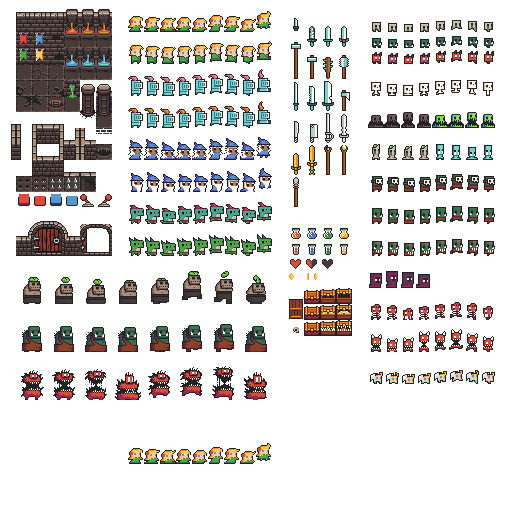
\includegraphics[width=0.5\textwidth]{dungeontiles.png}
\caption{\label{tiles}Tuiles du décor et personnages}
\end{center}
\end{figure}

\begin{figure}[h]
\begin{center}
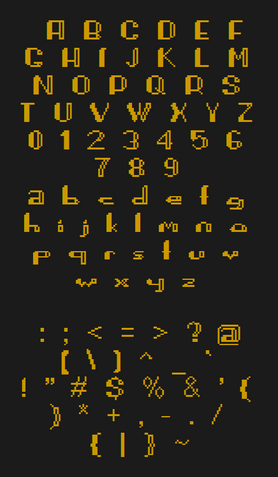
\includegraphics[width=0.5\textwidth]{font.png}
\caption{\label{font}Police de caractères}
\end{center}
\end{figure}

\clearpage
\section{Description et conception des états}

\subsection{Description des états}

Pour chacun des états du jeu, on retrouve une combinaison d'éléments fixes (la structure du labyrinthe) et d'éléments mobiles (personnage principal et ennemis).
Pour chaque élément, on comptera 2 propriétés que sont sa position et son identifiant (un id pour les murs, un pour les ennemis, le personnage principal ...).

\subsubsection{État éléments fixes}

Chaque étage du donjon possède un certain nombre fixe de cases. Toutes les cases ont un type parmi ces 4 : Mur, Espace (vide), Porte, Coffre.

Cases "Mur" (Wall) : Elles servent à délimiter les contours de chaque étage du donjon, les personnages ne pouvant pas les traverser.

Cases "Espace" (Space) : Il s'agit des cases sur lesquelles peuvent se déplacer librement les éléments mobiles, on trouve plusieurs sous-types de cases Espace :
- Une case de départ où apparaît le joueur.
- Une case de fin qui permet au joueur de passer à l'étage suivant (située après le boss de l'étage).
- Plusieurs cases "spawn" où apparaissent les ennemis.
- Des cases vides de tout élément.

Cases "Porte" (Door) : Ce sont des cases infranchissables par le joueur sauf si le joueur remplit les conditions requises (avoir tué un certain ennemi, avoir obtenu une clé ...), la case devient alors franchissable et donne accès à une nouvelle zone.

Cases "Coffre" (Chest) : Ce dernier type de case correspond à des cases qui permettent au joueur d'obtenir des éléments lui permettant de booster ses statistiques (Vitalité, Attaque ou Défense).

\subsubsection{État éléments mobiles}

Les éléments mobiles ont 3 caractéristiques, une direction (les 4 points cardinaux et une direction nulle), une vitesse et une position.
Lorsque la position est à 0 alors l'élément est exactement sur la case, sinon il se trouve entre sa case originale et la case qui correspond à sa direction, quand la position à la même valeur que la vitesse, le personnage se déplace dans la direction correspondante.

Nous avons défini 2 éléments mobiles que sont les ennemis (2 types pour le moment : Ghost, l'ennemi basique et Boss, l'ennemi plus puissant qui permet d'accéder à l'étage suivant) et le personnage principal (MainCharacter) qui n'est autre que le personnage contrôlé par le joueur.
Ces éléments mobiles ne disposent chacun que de 2 états : Alive et Dead, ils démarrent dans l'état Alive et passent à l'état Dead si leurs points de vie atteignent 0, pour les ennemis, ils disparaissent du jeu et pour le joueur, cela signifie la fin de la partie (donc le retour au 1er étage).
Comme détaillé dans la partie règle du jeu, ces éléments disposent de 3 caractéristiques sui déterminent leur puissance de combat (HealthPoints, Attack et Defense).

\subsubsection{État général}

On rajoute enfin 2 éléments généraux à ceux définis auparavant, il s'agit des variables epoch et epochRate.
La première sert simplement à connaître le nombre de "tour" depuis le début de la partie. 
La seconde permet de régler la vitesse du jeu en réglant le nombre d'époque par seconde.

\subsection{Conception Logiciel}

On peut voir notre diagramme des classes sur la page suivante (Figure x), on y retrouve donc toutes les classes mentionnées auparavant qui permettent de définir un état du jeu :
- MobileElement qui permet de définir des éléments mobiles et dont descendent les classes Monstre (ennemis) et MainCharacter (personnage jouable).
- StaticElement qui à le même rôle pour les éléments statiques qu'on retrouvera dans les étages de notre donjon : murs, portes, coffres ou espaces vides permettant aux personnages de se déplacer.
- State qui gère la vitesse du jeu et le nombre de tours effectués.
- Il y aussi de nombreuses classes dédiées à l'énumération de statuts ou de types.

Il reste donc 2 classes : 

Classe Element : Cette classe permet de définir chacun des éléments du jeu, qu'ils soient statiques ou mobiles. Ses seules caractéristiques sont des coordonnées (notés x et y) pour connaître la position de l'élément.

Classe ElementTab :  Comme son nom le laisse entendre, on a ici, un conteneur d'éléments qui n'est autre qu'un tableau en deux dimensions. Celui-ci contient donc l'intégralité des éléments dispersés sur un étage du donjon.
A noter que le conteneur principal est la classe State qui contient la totalité des données liées à un état donné.

\begin{landscape}
\begin{figure}[p]
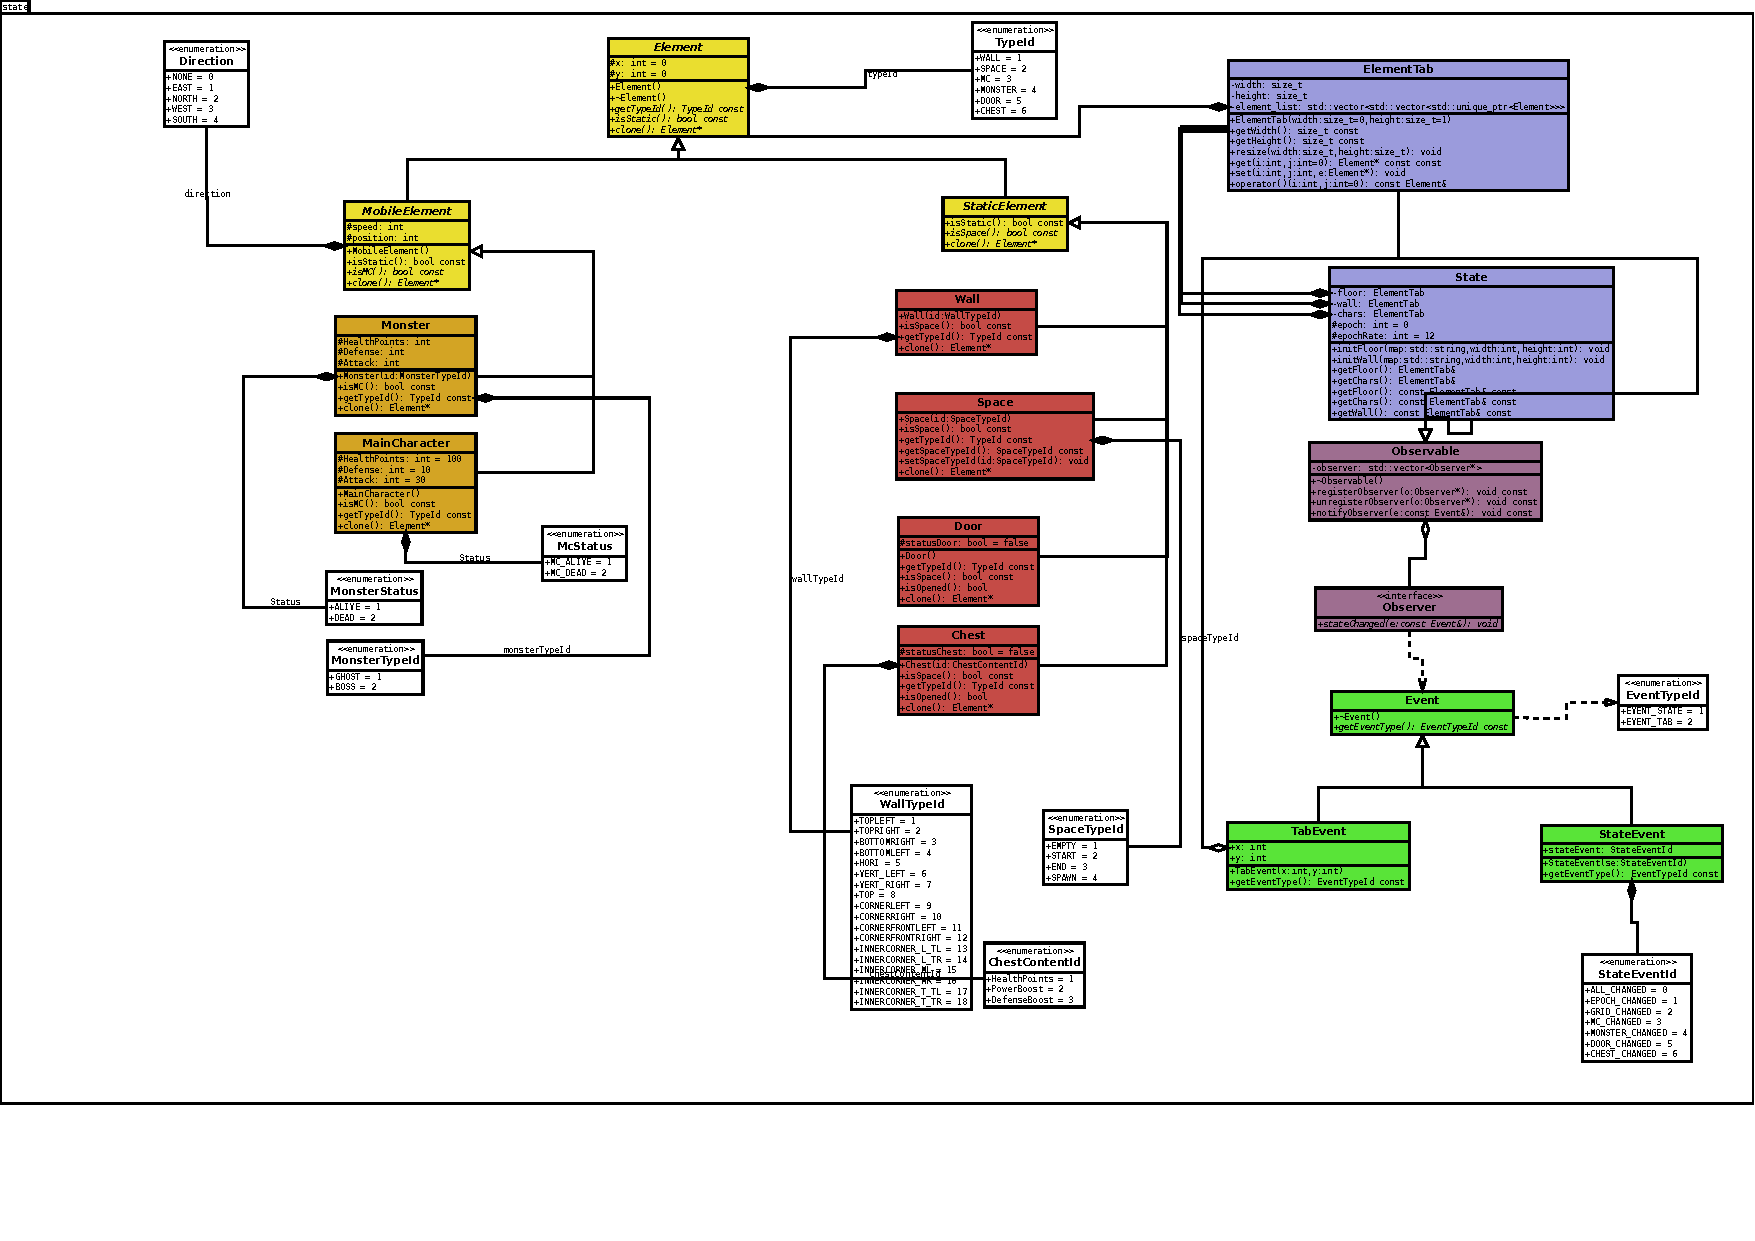
\includegraphics[width=0.9\paperheight]{state.pdf}
\caption{\label{uml:state}Diagramme des classes d'état.} 
\end{figure}
\end{landscape}

\clearpage
%\section{Rendu: Stratégie et Conception}
%
%\subsection{Stratégie de rendu d'un état}
%
%
%\subsection{Conception logiciel}
%
%%\begin{landscape}
%%\begin{figure}[p]
%%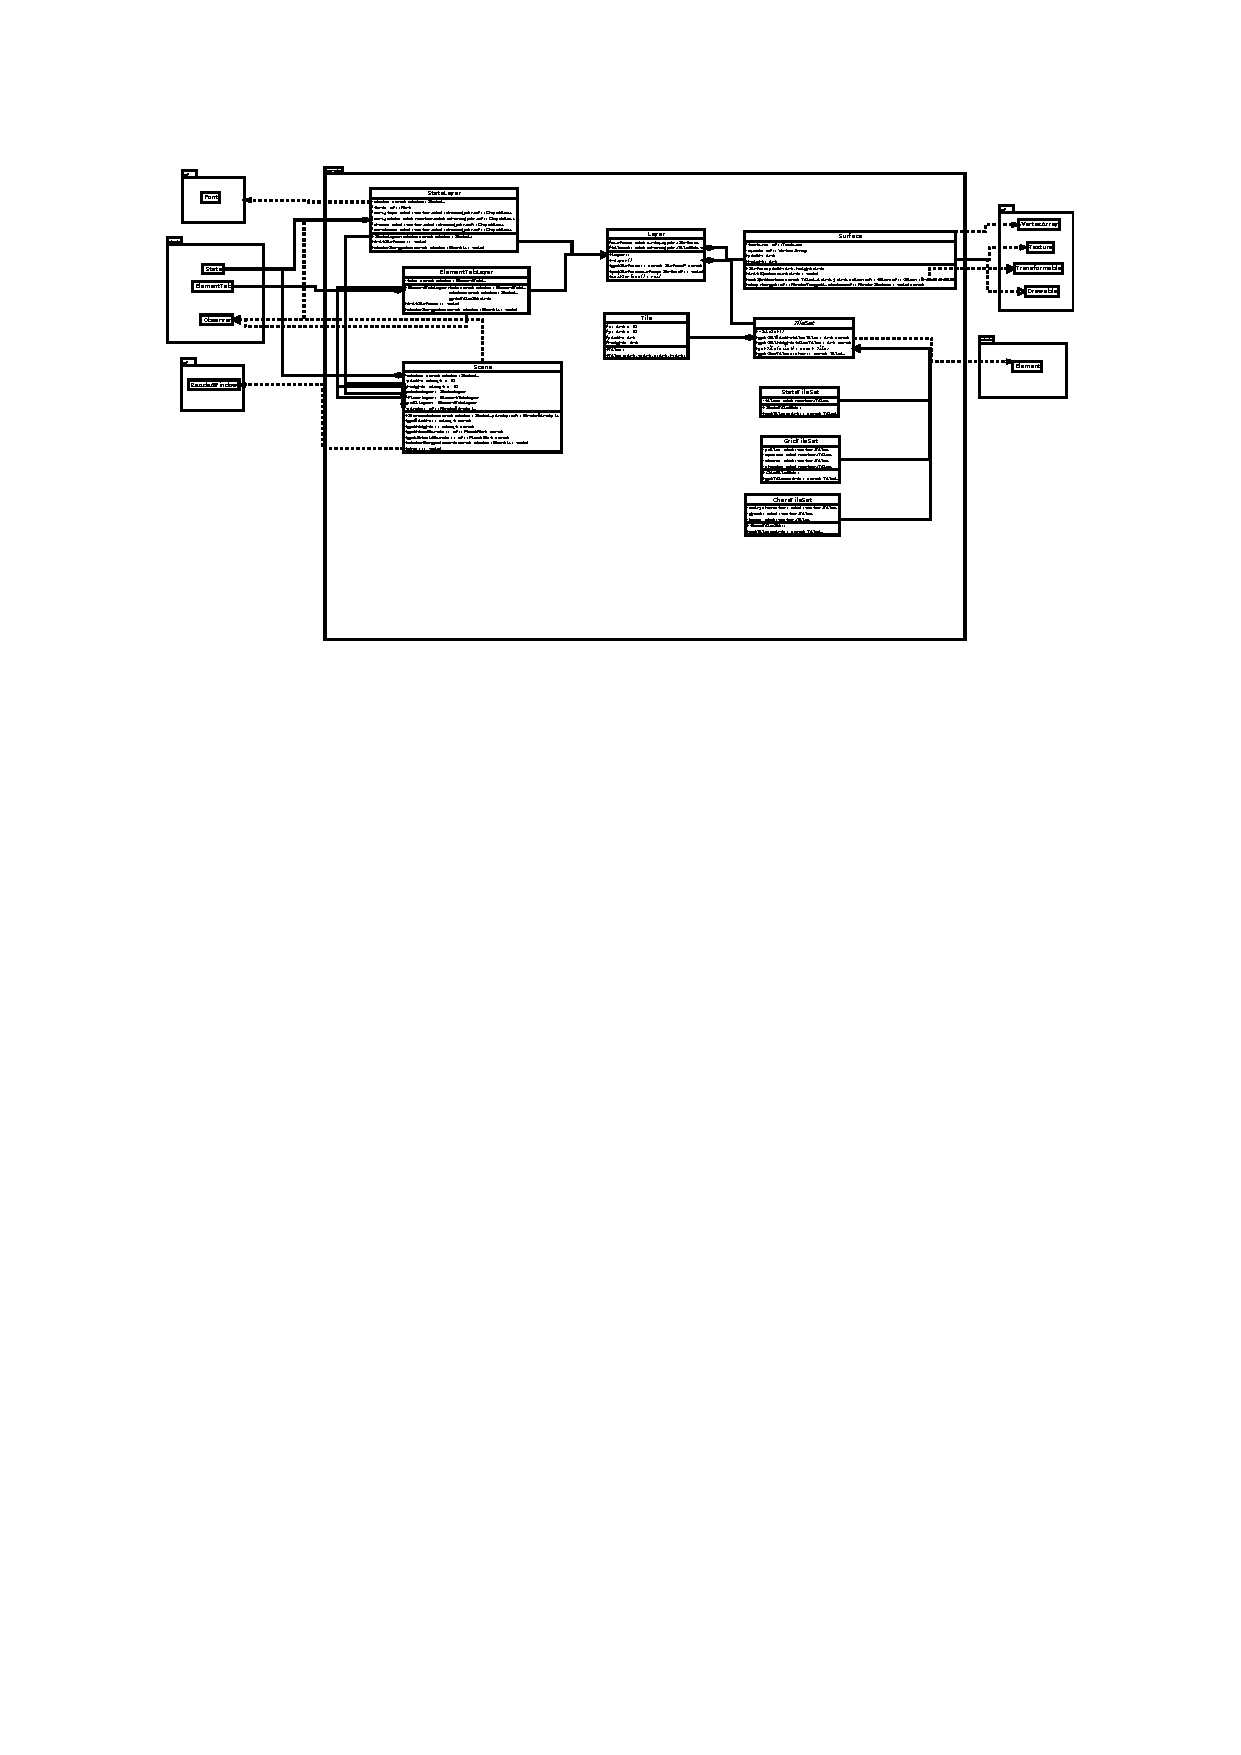
\includegraphics[width=0.9\paperheight]{render.pdf}
%%\caption{\label{uml:render}Diagramme des classes de rendu.} 
%%\end{figure}
%%\end{landscape}
%
%\clearpage
%\section{Règles de changement d'états et moteur de jeu}
%
%\subsection{Règles}
%
%\clearpage
%\subsection{Conception logiciel}
%
%
%%\begin{landscape}
%%\begin{figure}[p]
%%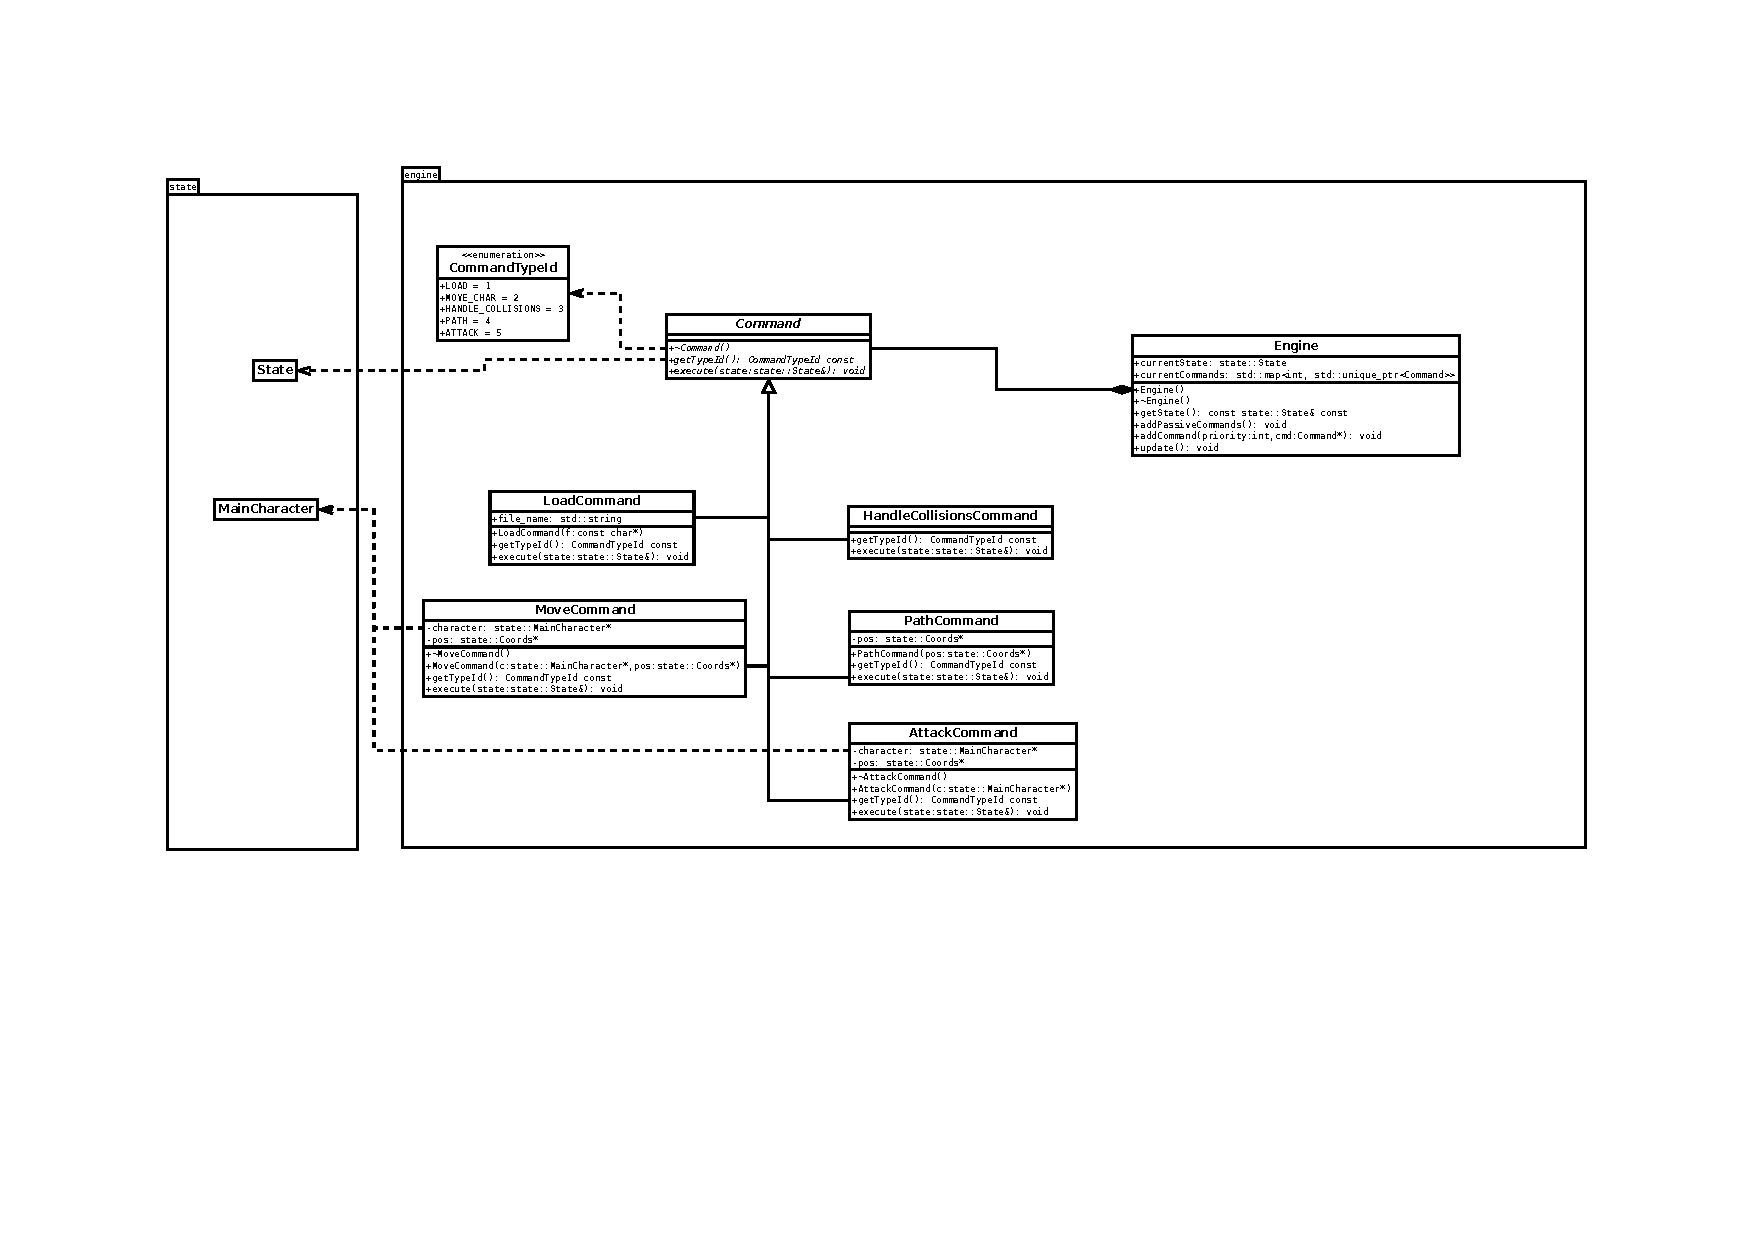
\includegraphics[width=0.9\paperheight]{engine.pdf}
%%\caption{\label{uml:engine}Diagramme des classes de moteur de jeu.} 
%%\end{figure}
%%\end{landscape}
%
%
%\section{Intelligence Artificielle}
%
%\subsection{Stratégies}
%
%\clearpage
%\subsection{Conception logiciel}
%
%
%%\begin{landscape}
%%\begin{figure}[p]
%%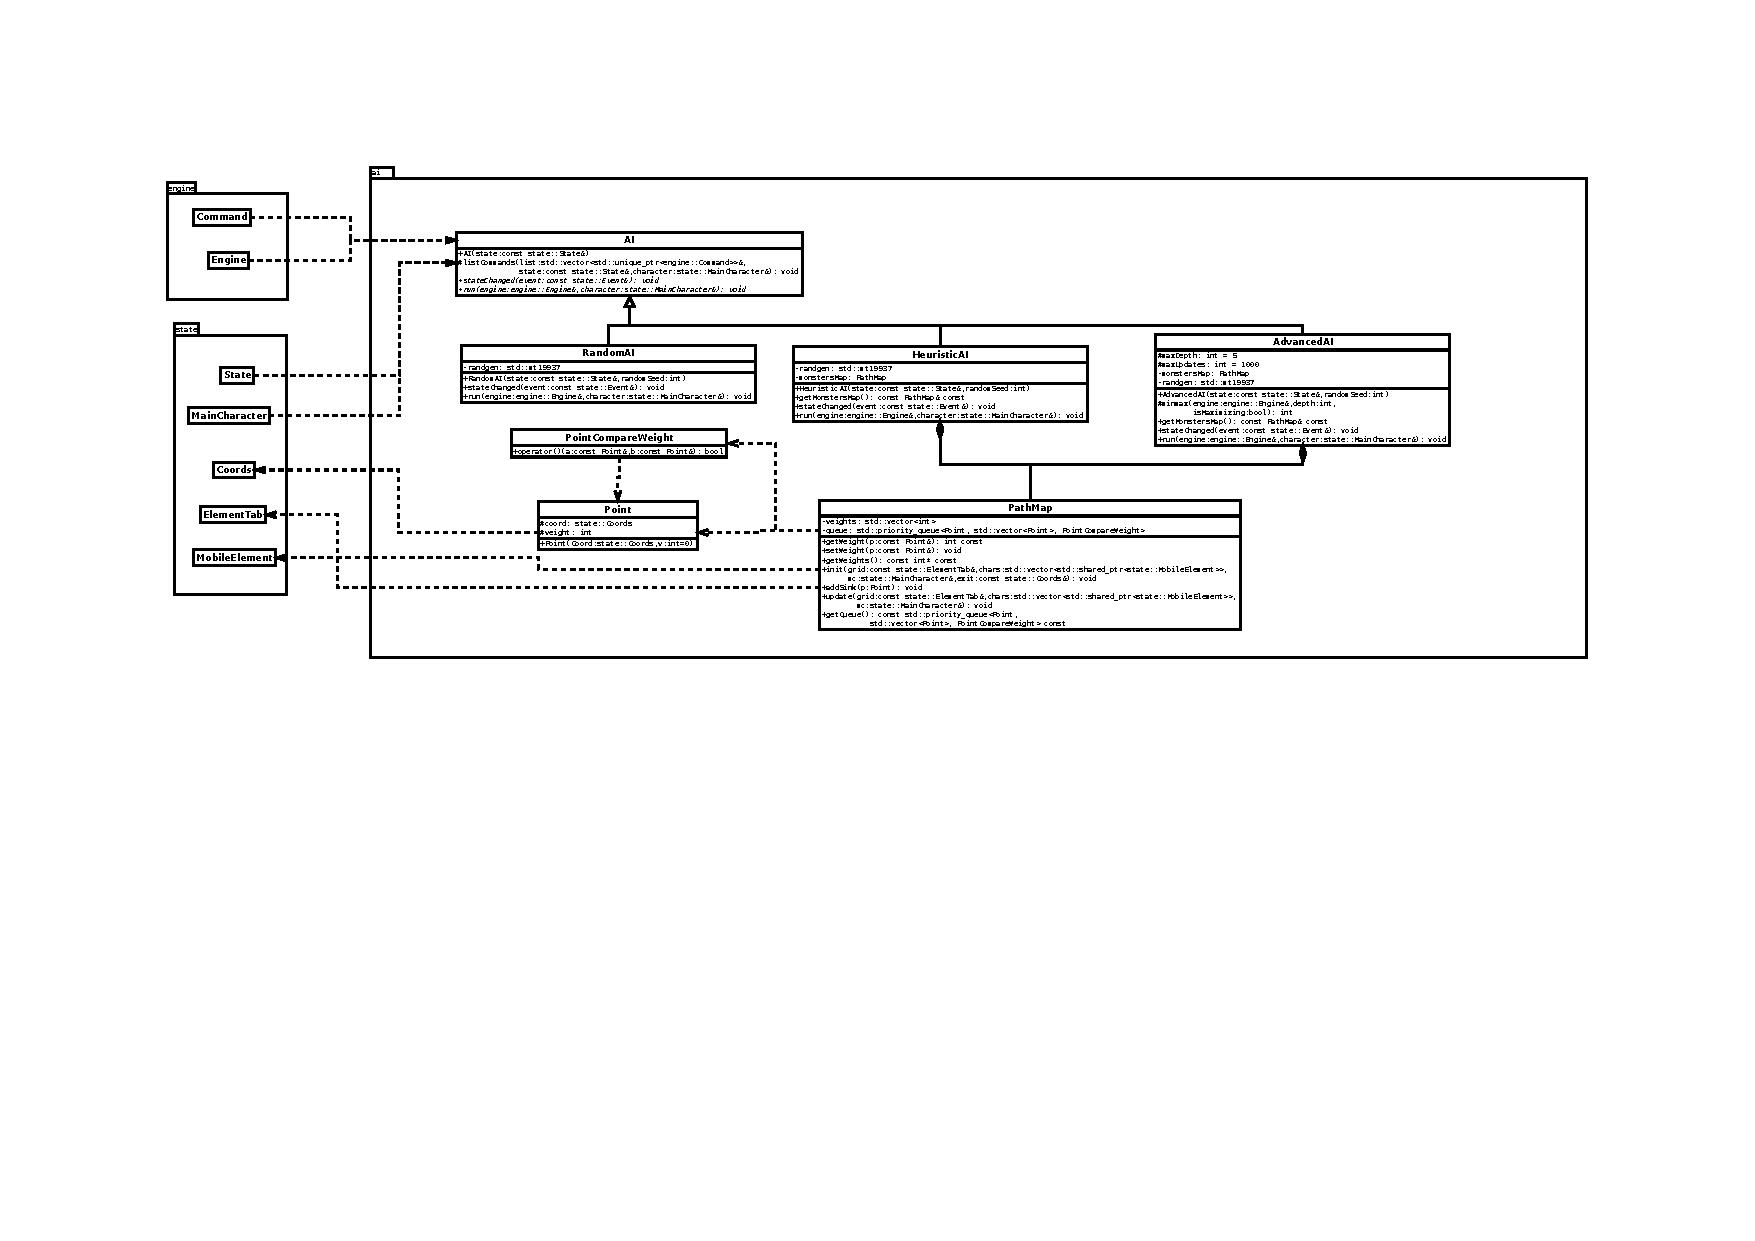
\includegraphics[width=0.9\paperheight]{ai.pdf}
%%\caption{\label{uml:ai}Diagramme des classes d'intelligence artificielle.} 
%%\end{figure}
%%\end{landscape}
%
%
%\section{Modularisation}
%\label{sec:module}
%
%\subsection{Organisation des modules}
%
%\clearpage
%\subsection{Conception logiciel}


%
%\begin{landscape}
%\begin{figure}[p]
%\includegraphics[width=0.9\paperheight]{module.pdf}
%\caption{\label{uml:module}Diagramme des classes pour la modularisation.} 
%\end{figure}
%\end{landscape}
 \addcontentsline{toc}{section}{Sources}
\section*{Sources}

\begin{itemize}
\item[Tiles :] DungeonTiles II \href{https://0x72.itch.io/dungeontileset-ii}{https://0x72.itch.io/dungeontileset-ii} par 0x72
\item[Font :] Pixel Font \href{https://devilsworkshop.itch.io/pixel-font}{https://devilsworkshop.itch.io/pixel-font


} par Ajay Karat | Devil's Work.shop
\end{itemize}

\end{document}
